%%%%%%%%%%%%%%%%%%%%%%%%%%%%%%%%%%%%%%%%%
% Uppsala University Assignment Title Page 
% LaTeX Template
% Version 1.0 (27/12/12)
%
% This template has been downloaded from:
% http://www.LaTeXTemplates.com
%
% Original author:
% WikiBooks (http://en.wikibooks.org/wiki/LaTeX/Title_Creation)
% Modified by Elsa Slattegard to fit Uppsala university
% License:
% CC BY-NC-SA 3.0 (http://creativecommons.org/licenses/by-nc-sa/3.0/)

%\title{Title page with logo}
%----------------------------------------------------------------------------------------
%	PACKAGES AND OTHER DOCUMENT CONFIGURATIONS
%----------------------------------------------------------------------------------------

\documentclass[12pt]{article}
\usepackage[english]{babel}
\usepackage[utf8x]{inputenc}
\usepackage{amsmath}
\usepackage{amssymb}
\usepackage{graphicx}
\usepackage{float}
\usepackage[normalem]{ulem}
\usepackage{tabularray}
\usepackage{color}
\usepackage{caption}
\usepackage{subcaption}
\usepackage{dsfont}
\usepackage{cite}
\usepackage{hyperref}
\usepackage[colorinlistoftodos]{todonotes}
\usepackage[ruled,vlined]{algorithm2e}
\usepackage{ragged2e}

\setlength {\marginparwidth }{2cm}
\newcommand{\tabitem}{~~\llap{\textbullet}~~}

\begin{document}
    \begin{titlepage}
    
    \newcommand{\HRule}{\rule{\linewidth}{0.5mm}} % Defines a new command for the horizontal lines, change thickness here
    
    \center % Center everything on the page
     
    %----------------------------------------------------------------------------------------
    %	HEADING SECTIONS
    %----------------------------------------------------------------------------------------
    
    \textsc{\LARGE{T\'{e}cnico Lisboa} \\ \vspace{0.5cm} \LARGE{University of Lisbon}}\\[1cm] % Name of your university/college
    \vspace{-2cm}
    \begin{figure}[H]
        \centering
        \begin{minipage}{.5\textwidth}
            \centering
            \phantom{............}
\includegraphics[width=.9\linewidth]{figures/logos/university-lisbon-logo.png}
        \end{minipage}%
        \begin{minipage}{.5\textwidth}
            \centering
            \hspace{-1cm}
            
\includegraphics[width=.9\linewidth]{figures/logos/tecnico-ulisboa-logo.png}
        \end{minipage}
    \end{figure}
    \vspace{-1cm}
     % Include a department/university logo - this will require the graphicx package
    \textsc{\Large Research Seminar in Information Security}\\[0.5cm] % Major heading such as course name
    \textsc{(Prof. Paulo \uppercase{Mateus})}\\[0.5cm]
    \textsc{Doctoral Program in Information Security}\\[0.5cm] % Minor heading such as course title
    \textsc{\large 2023/2024 - 1\textsuperscript{st} Semester}\\[0.5cm] % Minor heading such as course title
    
    %----------------------------------------------------------------------------------------
    %	TITLE SECTION
    %----------------------------------------------------------------------------------------
    
    \HRule \\[0.3cm]
        { \huge \bfseries Post-Quantum Security of \\  the (``tweakable'') \\ Even-Mansour Cipher \\ \vspace{0.5cm} \Large (Christian \textsc{\uppercase{Majenz}} - November 23, 2023)}\\[0.4cm] % Title of your document
    \HRule \\[1cm]
     
    %----------------------------------------------------------------------------------------
    %	AUTHOR SECTION
    %----------------------------------------------------------------------------------------
    
    \begin{minipage}{0.75\textwidth}
    
        \begin{flushleft} \large
            \textbf{Report written by:}\\
            \begin{itemize}
                \vspace{-0.1cm}
                \item \normalsize{Rúben \textsc{\uppercase{Barreiro}}:\\
                - \href{mailto:ruben.andre.letra.barreiro@tecnico.ulisboa.pt}{\emph{ruben.andre.letra.barreiro@tecnico.ulisboa.pt}}}
            \end{itemize}
        \end{flushleft}
    
    \end{minipage}\\[2cm]
    \vspace{-1cm}    
    % If you don't want a supervisor, uncomment the two lines below and remove the section above
    %\Large \emph{Author:}\\
    %John \textsc{Smith}\\[3cm] % Your name
    
    %----------------------------------------------------------------------------------------
    %	DATE SECTION
    %----------------------------------------------------------------------------------------
    
    {\large{Last updated: \today}}\\[2cm] % Date, change the \today to a set date if you want to be precise
    
    \vfill % Fill the rest of the page with whitespace

    \end{titlepage}

    \clearpage

    
    \section{Motivation}
    \label{sec:motivation}

    The task of interest in this seminar is to address the post-quantum security\break of the (``tweakable'') Even-Mansour Cipher through the combination of two previous experimental results, one of them on the security model of the plain Even-Mansour Cipher, as well as how to build variants of this cryptographic primitive considering also security models for the post-quantum setting \cite{alagic-et-al:post-quantum-security-tweakable-even-mansour-applications:2022:03-2024}.
    
    As a motivation quick start, nowadays, we are concerned about the known quantum attacks against the currently used modern cryptography, and there are different types of such attacks. First of all, we have what we can call post-quantum attacks on Asymmetric Cryptography (or Public Key Cryptography) \cite{merkle:secure-communications-over-insecure-channels:1975:03-2024,diffie-hellman:new-directions-cryptography:1976:03-2024}, such as the ones performed by the well-known Shor's\break algorithm \cite{shor:algorithms-quantum-computation-discrete-logarithms-factoring:1994:03-2024,shor:polynomial-time-algorithms-prime-factorization-discrete-logarithms-quantum-computer:1997:03-2024}, that completely break some cryptographic primitives such as Rivest-Shamir-Adleman (RSA)\cite{rivest-shamir-adleman:method-obtaining-digital-signatures-public-key-cryptosystems:1978:03-2024} and other based on Elliptic Curves \cite{miller:use-elliptic-curves-cryptography:1986:03-2024,koblitz:elliptic-curve-cryptosystems:1987:03-2024}\break and Discrete Logarithm problem \cite{elgamal:public-key-cryptosystem-signature-scheme-based-discrete-logarithms:1985:03-2024}. Then, we have other post-quantum\break attacks on Symmetric Cryptography \cite{rijmen-daemen:advanced-encryption-standard:2001:02-2024}, such as the ones performed by Grover's algorithm \cite{grover:fast-quantum-mechanical-algorithms-database-search:1996:03-2024} and other related ones \cite{simon:power-quantum-computation:1997:03-2024,brassard-hoyer-tapp:quantum-cryptanalysis-hash-claw-free-functions-1998:03-2024}, which do not break completely some of the currently used cryptographic primitives. However,\break Symmetric Cryptography is significantly impacted by these mentioned\break quantum algorithms since we can use these algorithms for (exhaustive) key search attacks against block ciphers or collision attacks against hash\break functions. On the other hand, once we know some specific cryptographic\break constructions very well, we can take classical attack strategies like differential\break and linear cryptoanalysis, and speed them up using Grover's algorithm\break \cite{kaplan-leurent-leverrier-naya-plasencia:quantum-differential-linear-cryptanalysis:2016:03-2024} for finding keys or collisions, which degrade the security of these\break cryptographic protocols, at least in principle despite we still do not know how to quantify that degradation of security. Finally, we have an additional class of quantum attacks, which we can call beyond post-quantum attacks, where we make some assumptions that are not justifiable in the usual use case for a symmetric key cryptographic algorithm. In this case, we assume the key is secret but that an attacker can access some pairs of plaintexts and ciphertexts\break while using a Known-Plaintext Attack (KPA) and exploiting quantum\break computing capabilities. These attacks could allow us to completely break specific cryptographic schemes, such as the Even-Mansour cipher \cite{even-mansour:construction-cipher-single-pseudorandom-permutation:1997:03-2024,dunkelman-keller-shamir:minimalism-cryptography-even-mansour-scheme-revisited:2012:03-2024} and some other block cipher modes of operation, in an unrealistic attack model.

    We are far less concerned about the security of Symmetric Cryptography against quantum attacks than the one for Asymmetric Cryptography, at least for pre-quantum Public Key Cryptography. However, we should still have a post-quantum security proof in the global settings for our security proofs.

    
    \section{(``Tweakable'') Even-Mansour Cipher}
    \label{sec:tweakable-even-mansour-cipher}

    The Even-Mansour cipher \cite{even-mansour:construction-cipher-single-pseudorandom-permutation:1997:03-2024,dunkelman-keller-shamir:minimalism-cryptography-even-mansour-scheme-revisited:2012:03-2024} is arguably one of the simplest possible\break block cipher constructions, on which we assume there is a public permutation $P$ that everybody can evaluate and should have some specific reasonable\break cryptographic properties. The block cipher operation of this cryptographic\break primitive requires a secret key $k$, and it starts by applying an eXclusive OR (XOR) operation on that secret key $k$ and a message $x$. Then, it applies the permutation $P$ to the previous intermediate result, followed by a new XOR operation on it and on the secret key $k$ again. This cryptographic scheme is an essential minimal construction because we can see a cipher as an oracle box we can evaluate forward and backward. For this reason, we need to have secret key $k$ before and after the permutation since it is breakable otherwise. Despite the simplicity of this cryptographic scheme, it represents a similar key aspect to the one used for real-world standardized symmetric cryptographic\break lightweight schemes such as Elephant \cite{beyne-chen-dobraunig-mennink:dumbo-jumbo-delirium-parallel-authenticated-encryption-lightweight-circus:2020:03-2024}, Chaskey \cite{mouha-et-al:chaskey-efficient-mac-algorithm-32-bit-microcontrollers:2014:03-2024}, and Minalpher \cite{sasaki-et-al:minalpher-v1:2014:03-2024}.

    \noindent Generally, we can describe the Even-Mansour cipher as follows. Given a public permutation $P: {\{0, 1 \}}^{n} \rightarrow {\{0, 1 \}}^{n}$ and a key $k \in {\{0, 1 \}}^{n}$, the cipher $E: {\{0, 1 \}}^{n} \times {\{0, 1 \}}^{n} \rightarrow {\{0, 1 \}}^{n}$ is defined as ${E}_{k} [P](x) = P(x \oplus k) \oplus k$. An illustrative sketch of the Even-Mansour cipher is given in the figure below:

    \begin{figure}[ht]
        \captionsetup{justification=centering}
        \centering
        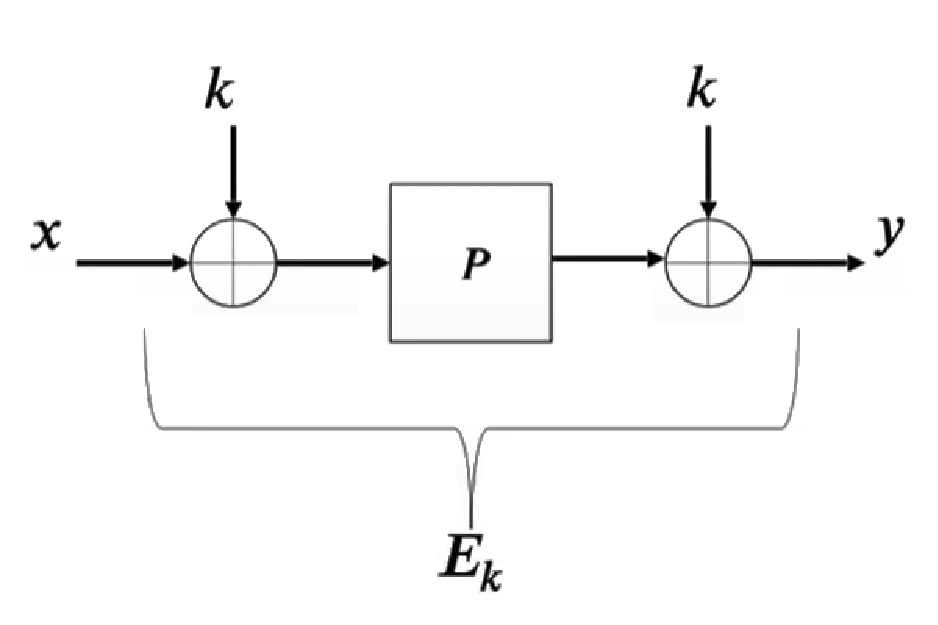
\includegraphics[width=0.5\textwidth]{figures/images/img-1.pdf}
        \caption{High-level illustration sketch of\\ the Even-Mansour cipher.}
    \end{figure}
    
    \noindent Furthermore, we can make this cryptographic construction a little more\break complicated and versatile by adding a simple extra input to the block cipher, which we usually call the ``tweak'' input $t$. This modification on the original block cipher should create a family of independent block ciphers dependent on this input $t$. Namely, for each different ``tweak'' $t$, we should obtain an independent block cipher while still only using one secret key $k$. Basically, in this new variant, we have a function $f(k,t)$ called the ``tweak'' function that fulfills few cryptographic properties, and for each random secret key, the output of this new block cipher is as good as the random and independent\break Even-Mansour keys used in the original block cipher. This feature can be helpful because, for some cipher mode operations, we can be concerned about length extension attacks, and we should apply a different operation in the last round of that cipher mode operation. In that case, we can use a different ``tweak'' input for the final round of the block cipher, for example. There are several applications of how to use this new ``tweak'' input $t$, and it is actually this new key ingredient of the (``tweakable'') Even-Mansour cipher that the previously mentioned symmetric key encryption schemes, such as Elephant \cite{beyne-chen-dobraunig-mennink:dumbo-jumbo-delirium-parallel-authenticated-encryption-lightweight-circus:2020:03-2024}, Chaskey \cite{mouha-et-al:chaskey-efficient-mac-algorithm-32-bit-microcontrollers:2014:03-2024}, and Minalpher \cite{sasaki-et-al:minalpher-v1:2014:03-2024} use in their constructions.

    \noindent Generally, we can describe the  ``tweak'' function used in the (``tweakable'') Even-Mansour cipher as follows. It is represented by a mathematical function $f: {\{0, 1 \}}^{{\ell}_{k}} \times \mathcal{T} \rightarrow {\{0, 1 \}}^{n}$ so that for a random key $k \leftarrow {\{0, 1 \}}^{{\ell}_{k}}$, the outputs $f(k, t)$ for different $t \in \mathcal{T}$ are as good as independent Even-Mansour keys. An illustrative sketch of the (``tweakable'') Even-Mansour cipher is given below:

    \begin{figure}[ht]
        \captionsetup{justification=centering}
        \centering
        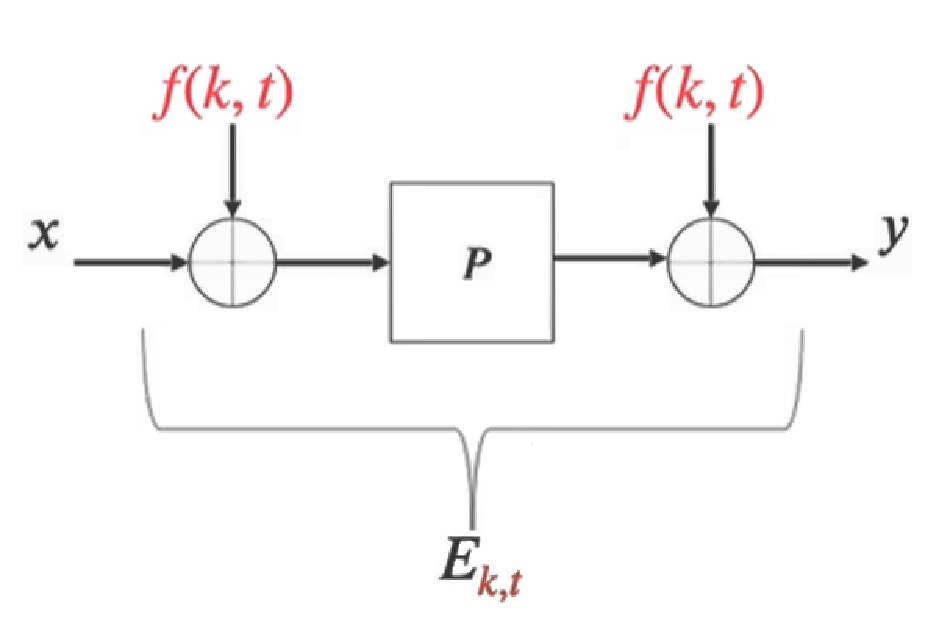
\includegraphics[width=0.5\textwidth]{figures/images/img-2.pdf}
        \caption{High-level illustration sketch of\\ the (``tweakable'') Even-Mansour cipher.}
    \end{figure}

    \noindent Then, we have an additional variant of this cryptographic primitive, which we know as the Even-Mansour Cipher with Key Expansion. Namely, this cryptographic primitive uses a shorter key $k$ of size $l$, which we expand using zero-padding of size $(n - l)$ and we permute the expanded bit string. Then, we apply the XOR operation with the input $x$ and the previous permuted result, permuting the output again before XORing it with the permutation of the shorter key expanded with zero-padding one last time. In this new variant,\break all the permutations used are the same permutations $P$ used for the original\break Even-Mansour cryptographic construction. However, we can conclude this cryptographic construction has both an advantage and a disadvantage. This cryptographic scheme is a bad idea because we always want to use different cryptographic primitives for distinct parts of a cryptographic construction. However, on the other hand, this same cryptographic scheme ends up being a great idea from a practical point of view because we can have different block lengths than the key lengths for some computational devices with Hardware acceleration for the permutation function $P$ if we only want to compute it.

    \noindent Generally, this Even-Mansour cipher with Key Expansion has a shorter key $k \in {\{0, 1 \}}^{\ell}$ and we can represent the respective cipher procedure $E$ as\break $E: {\{0,1\}}^{\ell} \times {\{0,1\}}^{n} \rightarrow {\{0,1\}}^{n}$. An illustrative sketch of this variant of Even-Mansour cipher with Key Expansion is given in the figure below:

    \begin{figure}[ht]
        \captionsetup{justification=centering}
        \centering
        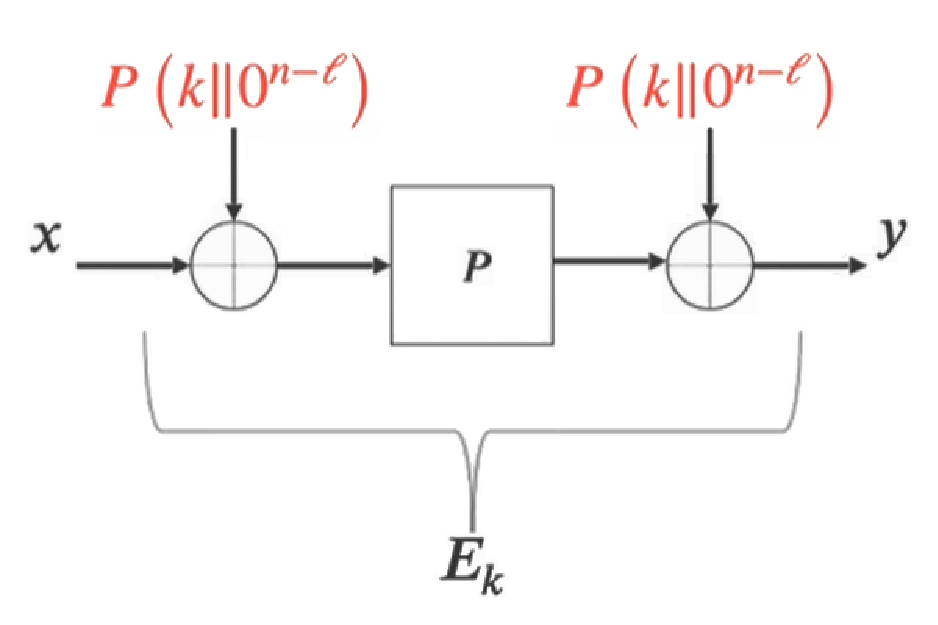
\includegraphics[width=0.5\textwidth]{figures/images/img-3.pdf}
        \caption{High-level illustration sketch of\\ the Even-Mansour cipher with Key Expansion.}
    \end{figure}

    \noindent Finally, we can combine the (``tweakable'') Even-Mansour Cipher with the Even-Mansour Cipher with Key Expansion. Then, considering the key\break expansion and permutation for the first input of the ``tweak function'', we end up with a more complex ``tweak function'' $f\left(t, P\left(k||{0}^{(n - \ell)}\right)\right)$. This feature\break keeps the cryptographic construction modular despite using this ``tweak'' function inside it not being sufficient to prove any post-quantum security yet.\break

    \noindent An illustrative sketch of the (``tweakable'') Even-Mansour cipher with Key Expansion, as a combination of the previous schemes, is given below:

    \begin{figure}[ht]
        \captionsetup{justification=centering}
        \centering
        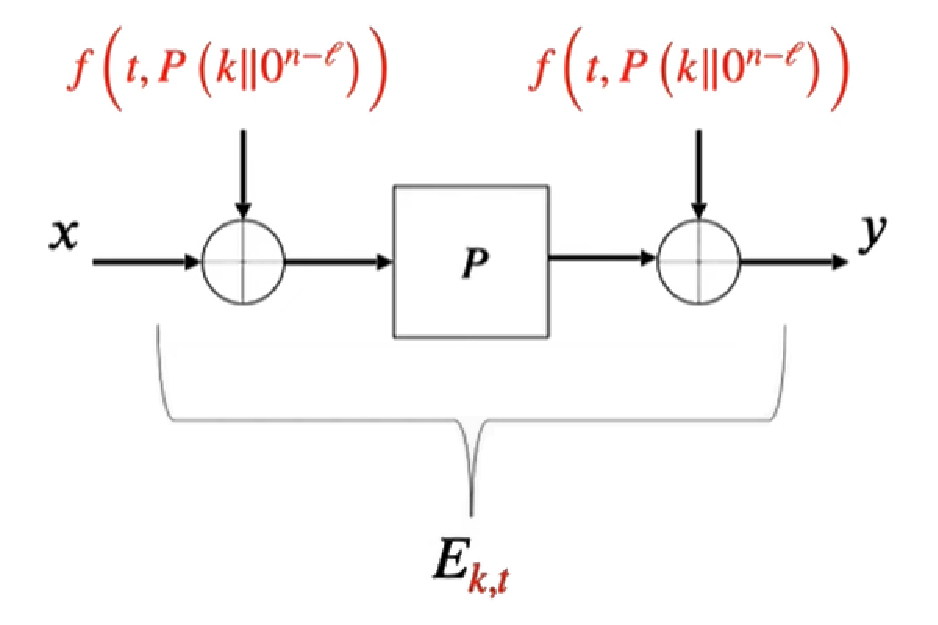
\includegraphics[width=0.5\textwidth]{figures/images/img-4.pdf}
        \caption{High-level illustration sketch of\\ the (``tweakable'') Even-Mansour cipher with Key Expansion.}
    \end{figure}

    
    \section{Attack Models}
    \label{sec:attack-models}

    There are three attack models: the classical attack model, the post-quantum attack model (also called the $Q1$ attack model), and the beyond post-quantum model (also called the $Q2$ attack model) \cite{kaplan-leurent-leverrier-naya-plasencia:breaking-symmetric-cryptosystems-using-quantum-period-finding:2016:03-2024,zhandry:how-construct-quantum-random-functions:2021:03-2024}. We can reason and argue about which attack model is the right one. The classical attack model is a\break little optimistic nowadays, and the beyond post-quantum attack model\break assumes the global community has considerably large access to quantum\break resources, which is unlikely since most of the devices we use daily are\break computational but they are not quantum ones. In fact, these cryptographic\break primitives based on the Even-Mansour block cipher fit more in the Lightweight Cryptography field, where the use cases are precisely the ones comprising\break the ubiquitous and mobile devices we use daily, following the trend of the\break Internet of Things (IoT). For these reasons, it is more reasonable to follow the\break post-quantum attack model, which is the case where we can evaluate this\break public permutation primitive $P$ on a quantum computer, but we only allow the construction of the Even-Mansour block cipher to be evaluated classically.

    
    \subsection{Security of the Even-Mansour Cipher}
    \label{subsec:security-even-mansour-cipher}

    For the security of the Even-Mansour Cipher, we start by idealizing the\break permutation $P$ as a uniformly random permutation. Now, we assume that some attacker makes a certain number of queries ${q}_{P}$ and ${q}_{E}$ on the public random permutation and the Even-Mansour Cipher, respectively, both in the forward and backward directions. For the classical attack model, we know that to break this block cipher classically, the product of the two numbers of queries must be in the order of ${2}^{n}$, i.e., ${q}_{P} \times {q}_{E} = \Omega({2}^{n})$ \cite{even-mansour:construction-cipher-single-pseudorandom-permutation:1997:03-2024}. Once we consider\break the unrealistic beyond post-quantum attack model, we can completely break this cryptographic scheme in theory since we can apply Simon's algorithm \cite{simon:power-quantum-computation:1997:03-2024} and attack this block cipher using only $\mathcal{O}(n)$ queries \cite{kuwakado-morii:security-quantum-type-even-mansour-cipher:2012:03-2024}. These observations\break make the security for the perspective of the post-quantum attack model much more frangible because we cannot argue without loss of generality that the attack performed is unitary once we are dealing with a mixture of oracles, where some of them have a quantum essence, and others have a classical one.

    
    \section{Experimental Results}
    \label{sec:experimental-results}

    For the experimental results, the author and his colleagues combined the previous results for (``tweakable'') Even-Mansour Cipher and Even-Mansour Cipher with Key Expansion \cite{alagic-et-al:post-quantum-security-tweakable-even-mansour-applications:2022:03-2024}. Namely, for an arbitrary Even-Mansour Cipher, we have the security bound given by the following expression:

    $$ 10 \cdot {2}^{-\frac{\hat{n}}{2}} \cdot \left( {q}_{P} \cdot \sqrt{{q}_{E}} + {q}_{E} \cdot \sqrt{{q}_{P}} \right) $$

    \noindent For the (``tweakable'') Even-Mansour cipher $E[P]$ (with or without Key\break Expansion), any quantum adversary making at most ${q}_{P}$ quantum queries to $P$ and ${q}_{E}$ classical queries to an oracle $O$ has distinguishing advantage between $O = E$ and $O = R$ at most the security bound given above. Here, $R$ is an independent (family of) random permutation and $\hat{n} = n$ ($\hat{n} = \ell$ for the Key Expansion variant). Additionally, ${q}_{P}$ and ${q}_{E}$ are again the number of queries made to the public random permutation and the Even-Mansour Cipher, respectively, while $\hat{n}$ is the key length for all cases. For the Key Expansion variant case, the key length is equal to the shorter key length ($\hat{n} = \ell$). Otherwise, the key length is equal to the block length used ($\hat{n} = n$).
    
    \noindent This experimental result was shown before for plain Even-Mansour Cipher \cite{jaeger-song-tessaro:quantum-key-length-extension:2021:03-2024} and is interesting in several contexts. First, this result is suitable when considering adversaries that decide on all the classical queries ahead of time, which is a non-adaptive choice on where to query. On the other hand, this experimental result is also sound for the realistic setting, where the number of queries to the key expansion construction is much smaller than the number of queries to the public random permutation. This last result is tight assuming\break ${q}_{E} \ll {q}_{P}$ and corresponds to cryptographic attacks based on solving the\break claw-finding problem. The security bound expression is also the success\break probability of an oracle that tries to distinguish the block cipher from a random permutation, which matches the one from the Brassard-Horne-Tapp (BHT) \cite{brassard-hoyer-tapp:quantum-cryptanalysis-hash-claw-free-functions-1998:03-2024} or ``offline'' Simon's \cite{simon:power-quantum-computation:1997:03-2024,bonnetain-et-al:quantum-attacks-without-superposition-queries-offline-simons-algorithm:2019:03-2024} algorithms. This security bound shows us we obtain the expected analog of the classical security for the key\break expansion case once we obtain the product of the two numbers of queries in\break the classical case, being equivalent to a collision \cite{wang-feng-lai-yu:collisions-hash-functions-md4-md5-haval-128-ripemd:2004:03-2024,stevens:fast-collision-attack-md5:2006:03-2024} or a claw-finding\break \cite{diffie-hellman:special-feature-exhaustive-cryptanalysis-nbs-data-encryption-standard:1977:03-2024,zhang:promised-distributed-quantum-search:2005:03-2024,tani:claw-finding-algorithms-using-quantum-walk:2009:03-2024} attack. For the ``tweakable'' case, the success probability is the same as the key expansion case. Additionally, for a fixed ``tweak'' input and a\break random secret key, the output needs to be random, while for two fixed but\break distinct tweaks and a random secret key, the XOR operation of the outputs still needs to be random. For those cases, a universal hash function such as the Carter-Wegman scheme \cite{carter-wegman:universal-classes-hash-functions:1977:03-2024,wegman-carter:new-hash-functions-their-use-authentication-set-equality:1981:03-2024} works as a good ``tweak'' function.

    
    \section{Proof Approach}
    \label{sec:proof-approach}

    Now, we can dive into the proof approach and the challenges that may occur when we try to prove the previous experimental results more in detail.

    
    \subsection{General Proof}
    \label{subsec:general-proof}

    In the classical setting, security proofs of Even-Mansour usually use what we can call global techniques. For example, these techniques may involve characterizing the probability that certain malicious and bad events happen that are defined globally for an entire transcript of queries. Another global technique commonly used is the $H$-coefficient technique, which also involves transcripts of queries, partitioning them into good and bad ones, and then comparing the expected results from the real world with the ideal world. In the quantum setting, we do not have transcripts of queries, and in particular, some techniques called Compressed Oracles can recover a kind of transcript of queries for the quantum setting. However, this technique is not available yet for random permutations. Therefore, what we can do is resort to a much ``more primitive'' technique, which turns out to be a more common technique in the quantum setting and that is referred to as the hybrid argument.

    
    \subsection{The Hybrid Argument}
    \label{subsec:hybrid-argument}

    Now, we can illustrate what happens when an adversary tries to break the (``tweakable'') Even-Mansour Cipher with Key Expansion, as shown below:

    \begin{figure}[ht]
        \captionsetup{justification=centering}
        \centering
        
        \vspace{-2ex}
        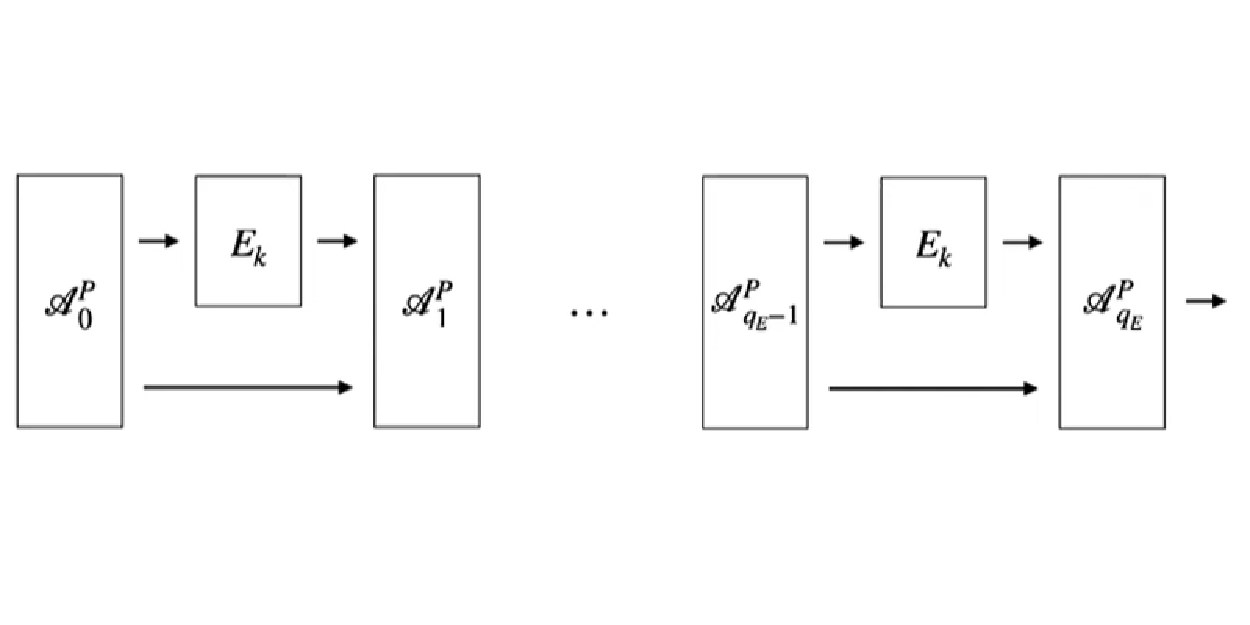
\includegraphics[width=0.95\textwidth]{figures/images/img-5.pdf}
        \vspace{-6ex}
        \caption{High-level illustration sketch of\\ the Hybrid Argument for an adversary having $({q}_{E} + 1)$ stages.}
    \end{figure}
    
    \noindent Namely, we can partition the adversary's actions in $({q}_{E} + 1)$ stages, basically as the phases before, between, and after the classical queries made to the block cipher. Thus, each one of these stages makes any arbitrary number of queries to the public permutation primitive $P$, which can be quantum queries, but the sum of those queries assumes some upper bound given by ${q}_{P}$. The naive hybrid approach consists of us replacing successively the block cipher ${E}_{k}$ with the idealized object stage by stage, which is an independent random permutation $R$. However, if we replace the block cipher ${E}_{k}$ with independent random permutations $P$ for the first couple of stages, the adversary could notice we changed the original cryptographic scheme. Therefore, we need to keep the future of the cryptographic scheme consistent with its ideal past in some sense, which represents a challenge in this proof. Luckily, what we can do in this situation is postpone the consistency problem until it disappears.

    \clearpage
    
    \noindent For the proof exploring the hybrid argument, we can design and introduce specific objects called hybrids, which are denoted as $H$ and shown below:

    \begin{figure}[ht]
        \captionsetup{justification=centering}
        \centering
        
        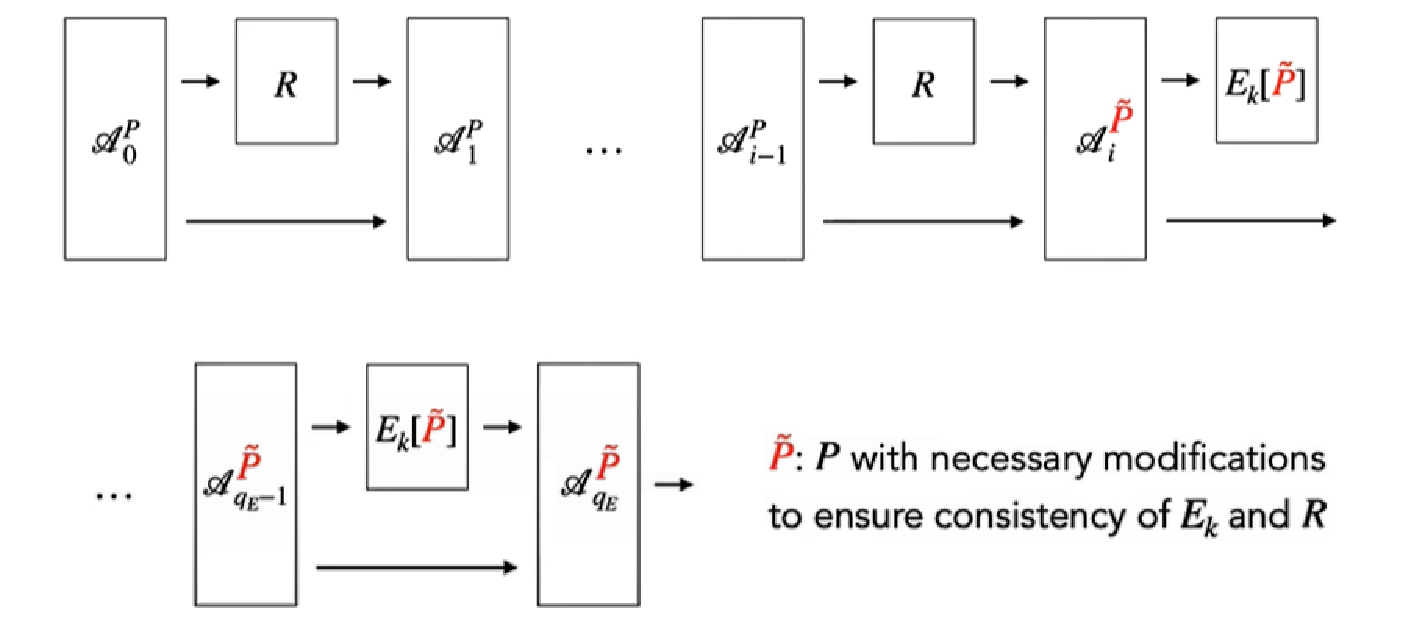
\includegraphics[width=0.95\textwidth]{figures/images/img-6.pdf}
        \caption{High-level illustration sketch of\\ the Hybrid objects for the security proof.}
    \end{figure}
    

    \noindent More specifically, for the first $i$ stages, we use these independent random permutations $R$, and then, we switch to the Even-Mansour Cipher in the end. But now, we slightly change the public random permutations $P$ to ensure the consistency of the cipher ${E}_{k}$ and independent random permutations $R$ with the previous queries made to the original scheme, from which we obtain a new random permutation $\tilde{P}$. Namely, this modified random permutation $\tilde{P}$\break blows up successively as the number of the first $i$ stages grows. However, there\break are also just a few applications for this modification, and in the end, in the last hybrid object, the effects of this modification disappear. Therefore, we do not have to worry about changing the public random permutations $P$ too much, once it works out for our general approach and how the proof proceeds.

    
    \section{Resampling Lemma Zoo}
    \label{sec:resampling-lemma-zoo}

    When we want to prove the indistinguishability property of these adjacent hybrid objects introduced before for this approach, we need to use some Resampling Lemmas, which we will describe in the following section in detail.

    
    \subsection{The Resampling Lemma for Functions}
    \label{subsec:resampling-lemma-functions}

    For simplicity reasons, we can start with the Resampling Lemma for random functions, where we have a uniformly random function $H$, which maps $n$ bits to other $n$ bits, and we have a two-stage algorithm $\mathcal{D}$ that plays a given interactive game with a challenger and a prover. This game starts with algorithm $\mathcal{D}$ interacting with some oracle to compute the random function $H$, outputting then some internal state. Then, the challenger samples a random bit $b$, jointly with two random bitstrings of size n denoted as ${x}^{*}$ and ${y}^{*}$. Now, we denote by ${H}_{({x}^{*} \mapsto {y}^{*})}$ the uniformly random function $H$ that we reprogram at the input ${x}^{*}$ to the output ${y}^{*}$. For $b = 0$, we do not perform any action, which gives us ${H}^{0} = H$, and for $b = 1$, we reprogram the function $H$ at the input ${x}^{*}$ to the output ${y}^{*}$. Then, in the second phase of this algorithm, we get access to this possibly changed $H$ function that gets ${x}^{*}$ as input, and the prover needs to decide if the ${H}^{b}$ function is the $H$ function reprogrammed at this input or not, choosing a $b'$ accordingly. The difficulty of winning this game is that ${x}^{*}$ is sampled at random by the challenger. The prover can gather as much information about $H$ as possible for $b = 0$, but if it does not query at ${x}^{*}$, it has no idea what the output should be, and it cannot detect if the challenger changed the corresponding output. Finally, the author and their colleagues proved that this simple case with a uniform random function provides a very sharp bound on the probability of winning this game \cite{grilo-hovelmanns-hulsing-majenz:tight-adaptive-reprogramming-qrom:2021:03-2024}. Namely, the probability of winning and distinguishing this game cannot be equal to $1$ unless the prover makes a number of queries on the order of ${2}^{n}$. A \break
    
    \clearpage
    
    \noindent simple illustration of this interactive proof game is given in the figure below:
    
    \begin{figure}[ht]
        \captionsetup{justification=centering}
        \centering
        
        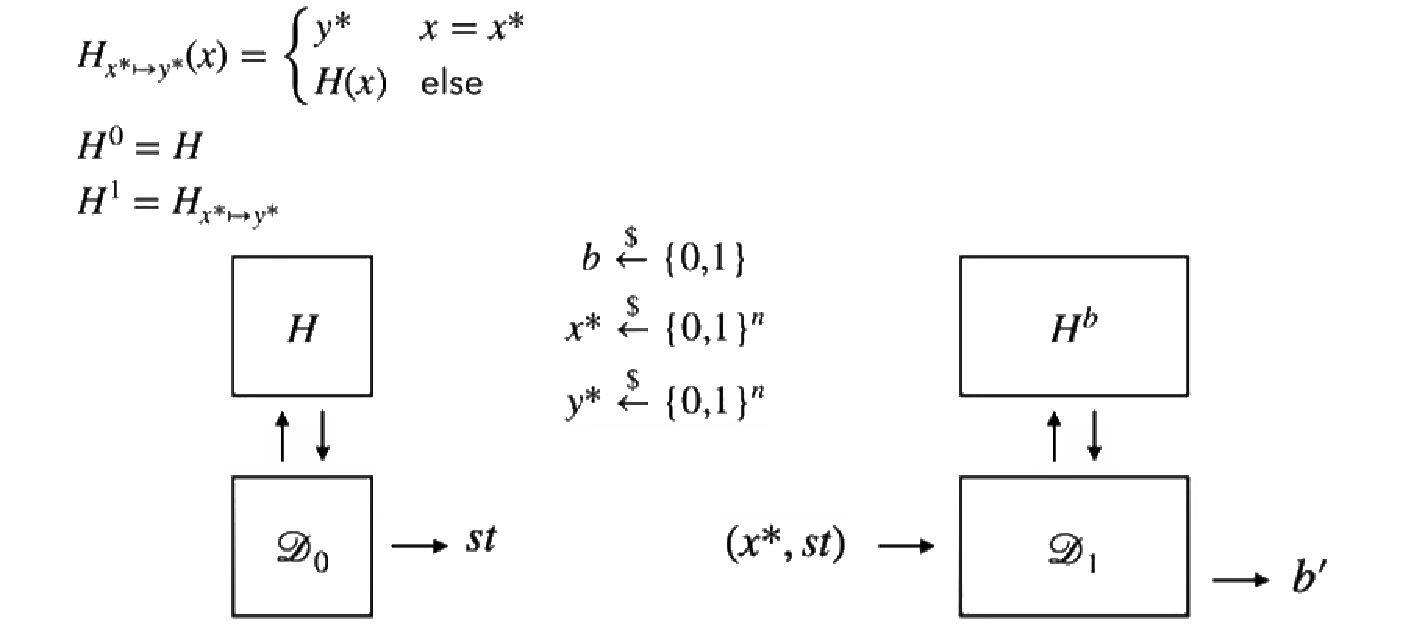
\includegraphics[width=0.8\textwidth]{figures/images/img-7.pdf}
        \caption{High-level illustration sketch of\\ the Interactive Proof Game for\\ the Resampling Lemma for Functions.}
    \end{figure}
    
    
    \noindent The bound for the probability of winning this interactive game is given as:

    $$ Pr[\mathcal{D}\ wins] \leq \frac{1}{2} + \frac{3}{2} \cdot \sqrt{{q}_{0} \cdot {2}^{-n}} $$

    \vspace{4ex}
        
    \subsection{The Resampling Lemma for Permutations}
    \label{subsec:resampling-lemma-permutations}

    For the case of permutations, we want to take a similar approach to what we follow for random functions. However, if we take a random input and reprogram the permutation to a random output, we are no longer dealing with a random permutation. Thus, keeping track of what is happening becomes extremely hard when we follow that approach using the hybrid argument. In the end, it is preferable to keep the permutation property and follow again a two-phase interactive game. In the first phase, also known as the learning phase, instead of resampling a new output, the challenger picks two inputs, ${s}_{0}$ and ${s}_{1}$, jointly with a random bit $b$ again. If $b = 0$, the challenger does not perform any action again. Otherwise, if $b = 1$, the challenger switches the outputs for these two picked inputs. Note that we know if $b = 0$, the challenger chooses the actual permutation we want to reprogram, and it picks ${s}_{0}$ and ${s}_{1}$ at random. Actually, the challenger has reprogrammed the output at the inputs ${s}_{0}$ and ${s}_{1}$ to a uniformly random output for $b = 0$ because it picked ${s}_{0}$ and ${s}_{1}$ uniformly random. Now, the challenger needs to finish the game, and as expected, the prover gets the two resembling inputs and tries to guess the bit $b$ used, similar to what we defined for the case of random functions. For this case, the probability of winning the game (and respective security bound) is essentially the same as in the case of random functions \cite{alagic-bai-katz-majenz:post-quantum-security-even-mansour-cipher:2021:03-2024}.
        
    
    \noindent An illustration of this interactive challenge-proof game is given below:
    
    \begin{figure}[ht]
        \captionsetup{justification=centering}
        \centering
        
        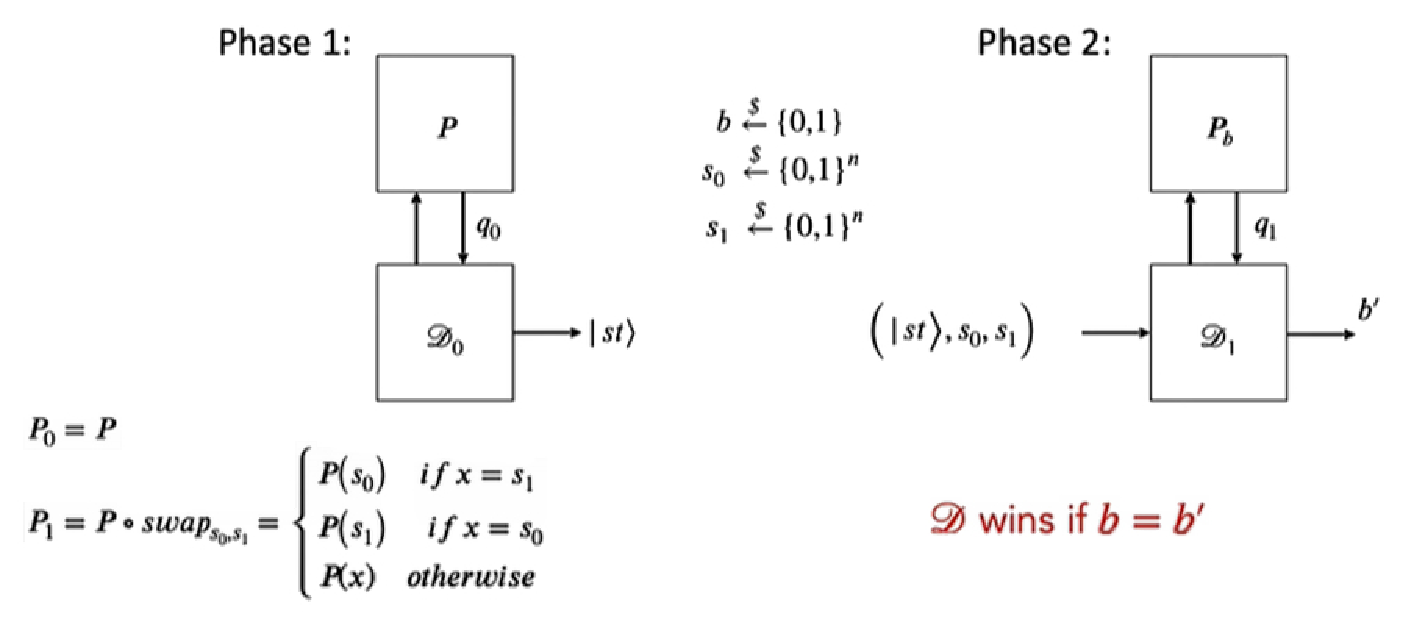
\includegraphics[width=0.9\textwidth]{figures/images/img-8.pdf}
        \caption{High-level illustration sketch of\\ the Interactive Proof Game for\\ the Resampling Lemma for Permutations.}
    \end{figure}

    
    \noindent The bound for the probability of winning this interactive game is given as:

    $$ Pr[\mathcal{D}\ wins] \leq \frac{1}{2} + 2 \cdot \sqrt{{q}_{0} \cdot {2}^{-n}} $$

    \vspace{4ex}
    
        
    \subsection{\mbox{The Resampling Lemma for}\break Key Expansion}
    \label{subsec:resampling-lemma-key-expansion}

    Finally, if we consider the Even-Mansour Cipher variant with the additional\break Key Expansion step, the proof for indistinguishability becomes much more\break complicated. In this case, we start again with the learning phase, but now we are more constrained on what we can do. Namely, we allow the adversary to output a distribution $\mathcal{D}$ and a parameter $\tau$. The adversary outputs the distribution $\mathcal{D}$, according to which we should sample the input $\hat{s}$ where we disorder with the uniformly random public permutation $P$. The adversary also outputs the parameter $\tau$, which represents a form of post-processing of the sample after expanding it through the public random permutation $P$.
    
    
    \noindent An illustration of this interactive challenge-proof game is given below:
    
    \begin{figure}[ht]
        \captionsetup{justification=centering}
        \centering
        
        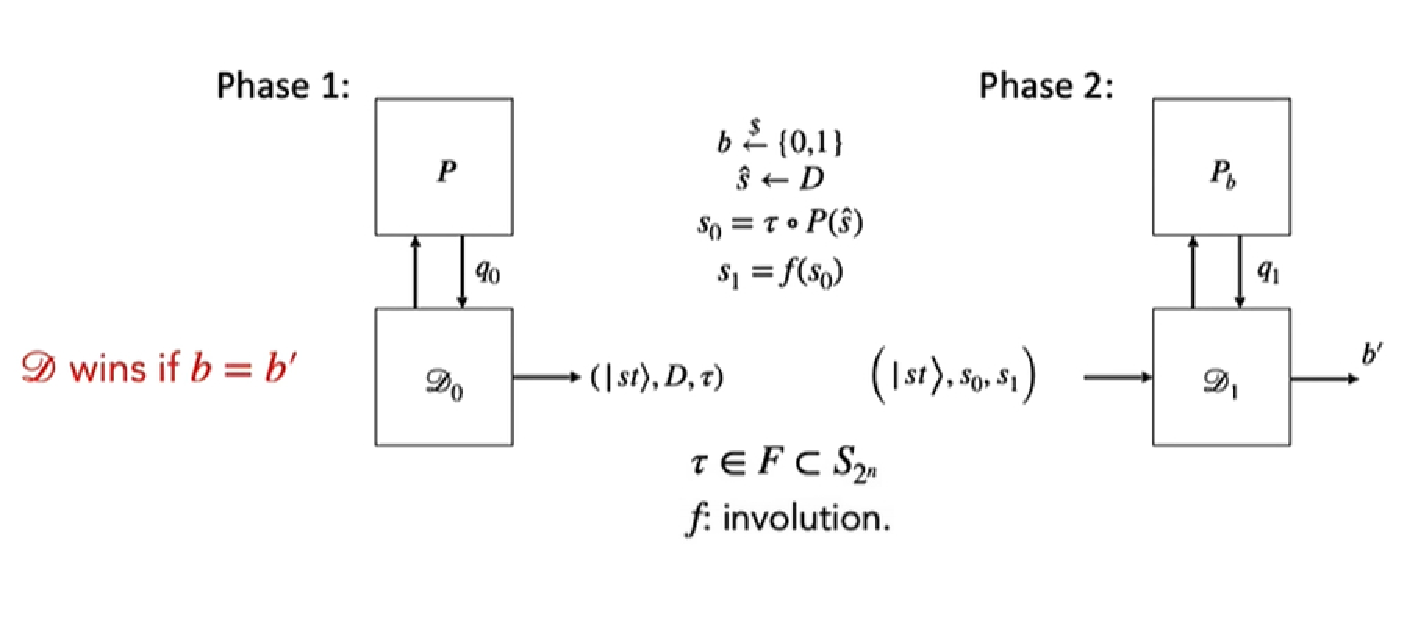
\includegraphics[width=0.9\textwidth]{figures/images/img-9.pdf}
        \caption{High-level illustration sketch of\\ the Interactive Proof Game for\\ the Resampling Lemma for Key Expansion.}
    \end{figure}
    
    
    \noindent Now, the adversary has a lot of choices regarding how the challenger should pose the challenge, and we need to choose $\tau$ from a subset of all permutations.\break Otherwise, the security bound will not be good enough, and the ``tweak\break function'' $f$ should represent an involution of pairs of ${s}_{0}$ and ${s}_{1}$. The prover should decide this pairing ahead of time. However, since we have this very restricted setting, then even though the sampling of the inputs involves the public random permutation $P$ itself and the adversarial actions, we still can obtain the following upper bound for the probability of winning\break the interactive proof game, which represents the security bound itself \cite{alagic-et-al:post-quantum-security-tweakable-even-mansour-applications:2022:03-2024}:

    $$ Pr[\mathcal{D}\ wins] \leq \sqrt{\epsilon} \cdot \left( 1 + \sqrt{q + \log\left( \frac{11 \cdot |F|}{\sqrt{\epsilon}} \right)} \right) $$

    \vspace{2ex}

    \centering
    \noindent Where:
    $$ \epsilon = \max_{s}\ \underset{({s}_{0}, {s}_{1}) \leftarrow \mathcal{D}}{Pr}\ \ [s = {s}_{0} \vee s = {s}_{1}] $$

    \justifying
    \noindent In this security bound, the most complex part of the mathematical expression is on logarithmic order. At the same time, $\epsilon$ is the minimal entropy of the distribution $\mathcal{D}$ to sample $\hat{s}$ because it is the adversary that provides it.

    \section{Superposition Oracle Resampling}
    \label{sec:superposition-oracle-resampling}

    Now, to prove these resamplings for both random function and permutation cases, we need to introduce the notion of superposition oracle resampling \cite{zhandry:how-record-quantum-queries-applications-quantum-indifferentiability:2018:03-2024}.
    
    \subsection{Superposition Oracle Resampling for Functions}
    \label{subsec:superposition-oracle-resampling-functions}

    For the case of functions, we use these superposition oracles where we have a random function for the ``vanilla'' random oracle, and we have a superposition\break of functions for the superposition oracle. Namely, in this last oracle, for each function output, we have a separate quantum register that is initialized in the uniform superposition of states to represent the uniform function output.\break For the superposition oracle, instead of having this fixed query unitary as in the ``vanilla'' random oracle, we have a controlled unitary that reads out this appropriate quantum register and answers the query that way. Finally,\break resampling for the superposition oracle is very similar to the case of the ``vanilla'' random oracle, with random input and output, using as well the reprogramming step. However (and luckily), we can discard (or reset) the\break appropriate quantum register ${F}_{{x}^{*}}$ and initialize it in a new uniform quantum\break superposition of states, resulting now in our new resampling operation, since\break the classical resampling is just sample a fresh independent output for which we can use an independent uniform quantum superposition state. Then, we conclude this set of steps is sufficient for achieving the core argument of\break replacing this Oracle distinguishability task with a state discrimination task, where we need to discriminate the original quantum state of the oracle\break simulation from the one where we replaced this uniform quantum\break superposition. This resampling works because, after just a few queries, most of the quantum registers intuitively contain the initial quantum state. After all, the adversary has only looked at $q$ many inputs (and queries), even if it uses a quantum superposition of states to perform such query operations. 
    
    \clearpage

    
    \vspace{-4ex}
    \noindent We now show a global overview of the main differences between the random function oracle and the superposition oracle for random functions below:
    
    \begin{table}[htp]
        \centering
        \resizebox{0.8\columnwidth}{!}{
            \begin{tblr}{
                width = \linewidth,
                colspec = {Q[535]Q[408]},
                row{3} = {c},
                row{13} = {fg=black},
                cell{1}{1} = {c=2}{0.943\linewidth},
                vline{2} = {5-13}{},
                cell{15}{1}={c=2}{},
                cell{16}{1}={c=2}{},
                cell{17}{1}={c=2}{},
                }
                $H: {\{0,1\}}^{n} \rightarrow {\{0,1\}}^{n}$ & \\
                & \\
                \textbf{Random Function Oracle} & \textbf{Quantum Superposition Oracle \cite{zhandry:how-record-quantum-queries-applications-quantum-indifferentiability:2018:03-2024}}\\
                & \\
                & \\
                For each $x \in {\{0,1\}}^{n}$: & For each $x \in {\{0,1\}}^{n}$:\\
                ~ ~ $H(x) \leftarrow {\{0,1\}}^{n}$ & {\phantom{....}Initialize $n$-qubit\\\phantom{....}quantum register ${F}_{x}$ in\\\phantom{....}the quantum state\\\phantom{....}$|{\phi}_{0}\rangle = {|+\rangle}^{\oplus n}$}\\
                & \\
                \textbf{Query Unitary}: & \textbf{Query Unitary}:\\
                ~ ~ ${U}_{H} {|x\rangle}_{X} {|y\rangle}_{Y} = {|x\rangle}_{X} {|y \oplus H(x)\rangle}_{Y}$ & ~ ~ $O{|x\rangle}_{X} = {CNOT}_{{F}_{x}:Y}^{\oplus n}$\\
                & \\
                \textbf{Resampling at ${x}^{*}:{y}^{*} \leftarrow {\{0,1\}}^{n}$}, & {\color{black}\textbf{Resampling at ${x}^{*}$}: \vspace{1ex}\\  \color{red}\phantom{..}\tabitem Discard the contents of\\\phantom{......} the quantum register ${F}_{{x}^{*}}$;\\ \phantom{..}\tabitem Prepare the exact same\\\phantom{......} quantum register ${F}_{{x}^{*}} $ in\\ \phantom{......} the quantum state $|{\phi}_{0}\rangle$;} \\
                \vbox{
                    \vspace{-15ex}    
                    \begin{equation*}
                        \vspace{10ex}
                        \hspace{-5ex}
                        H'(x) = \begin{cases}
                            {y}^{*}, & \text{if $x = {x}^{*}$}.\\
                            H(x), & \text{otherwise}.
                        \end{cases}
                    \end{equation*}
                } & \\
                & \\
                Most quantum registers are in the quantum state ${|+\rangle}^{\oplus n}$ after $q$ queries... \\
                \color{red}$\Rightarrow$ Distinguish quantum states resampled or not $\rightarrow$ Quantum State\color{black}\\
                \phantom{..................................................................................}\color{red}Discrimination (QSD)\color{black}\\
            \end{tblr}
        }
        \label{tab:global-overview-main-differences-between-random-function-oracle-and-quantum-superposition-oracle}
        \caption{\centering Global Overview of the main differences between\break the Random Function Oracle and Quantum Superposition Oracle.}
    \end{table}

    
    \subsection{Superposition Oracle Resampling for Permutations}
    \label{subsec:superposition-oracle-resampling-permutations}

    For the case of permutations, we still use a superposition oracle similar to the one used for the case of functions. However, we initialize it in a uniform\break quantum superposition of all function tables for a permutation. The query unitary is the same as the case of functions, but now we need a more intricate way of resampling, where we choose two uniformly random inputs and swap their outputs. In this case, we cannot take the same action as for the case of functions and discard some registers, initializing them then from scratch, since we will not end up with a permutation in that case. So, the technique we adopt for this case is to prove the resampling lemma in the ``Heisenberg\break Picture'', and we show that the reprogramming operation essentially almost commutes with the superposition oracle calls of the adversary, at least if the input is honest. We show an overview of the differences between the random permutation oracle and the superposition oracle for permutations below:
    
    \begin{table}[htp]
        \centering
        \resizebox{0.86\columnwidth}{!}{
            \begin{tblr}{
                width = \linewidth,
                colspec = {Q[535]Q[408]},
                row{3} = {c},
                row{13} = {fg=black},
                cell{1}{1} = {c=2}{0.943\linewidth},
                vline{2} = {5-12}{},
                cell{14}{1}={c=2}{},
                cell{15}{1}={c=2}{},
                }
                $P \in {S}_{{2}^{n}}$ & \\
                & \\
                \textbf{Random Permutation Oracle} & \textbf{Quantum Superposition Oracle}\\
                & \\
                & \\
                $P \leftarrow {S}_{{2}^{n}}$ & {Initialize ${2}^{n} \cdot n$-qubit\\ quantum register $F$ in\\ the quantum state\\ $|{\phi}_{0}\rangle = \frac{1}{\sqrt{{2}^{n}!}} \sum_{\pi \in {S}_{{2}^{n}}} |\pi({0}^{n})\rangle$\\\phantom{............................~~}$|\pi({0}^{(n - 1)}1)\rangle$\\\phantom{............................~~}$\dots |\pi({1}^{n})\rangle$}\\
                & \\
                \textbf{Query Unitary}: & \textbf{Query Unitary}:\\
                ~ ~ ${U}_{P} {|x\rangle}_{X} {|y\rangle}_{Y} = {|x\rangle}_{X} {|y \oplus P(x)\rangle}_{Y}$ & ~ ~ $O{|x\rangle}_{X} = {CNOT}_{{F}_{x}:Y}^{\oplus n}$\\
                & \\
                \textbf{Resampling at $({s}_{0},{s}_{1}): b \leftarrow \{0,1\}$}, & {\color{black}\textbf{Resampling at $({s}_{0},{s}_{1})$}: \vspace{1ex}\\  \color{red}\phantom{..}???\color{black}} \\
                \vbox{
                    \vspace{-4ex}    
                    \begin{equation*}
                        \hspace{-5ex}
                        P'(x) = \begin{cases}
                            {s}_{(i - b)}, & \text{if $x = {s}_{i}$}.\\
                            P(x), & \text{otherwise}.
                        \end{cases}
                    \end{equation*}
                } \\
                & \\
                Prove in ``Heisenberg Picture'' instead: \\
                \color{red}$\left[ {Swap}_{{F}_{{s}_{0}}{F}_{{s}_{1}}},{O}_{XYF} {\left( {P}_{{s}_{0}{s}_{1}} \right)}_{X} \right] = 0$, ${P}_{{s}_{0}{s}_{1}} = \mathds{1} - |{s}_{0}\rangle\langle{s}_{0}| - |{s}_{1}\rangle\langle{s}_{1}|$\color{black}\\
            \end{tblr}
        }
        \label{tab:global-overview-main-differences-between-random-permutation-oracle-and-quantum-superposition-oracle}
        \caption{\centering Global Overview of the main differences between\break the Random Permutation Oracle and Quantum Superposition Oracle.}
    \end{table}

    \clearpage
    
    \subsubsection{Superposition Oracle Resampling for Permutations used in Key Expansion}
    \label{subsubsec:superposition-oracle-resampling-permutations-key-expansion}

    Finally, we have the case of permutations used in the key expansion variant of the Even-Mansour Cipher, which is the most complicated case. In this case, we want to use the previously mentioned commutation result, where\break the resampling operation approximately commutes with the superposition oracle calls made by the adversary. However, note the inputs ${s}_{0}$ and ${s}_{1}$, which show up in this commutator equality, are sampled conditioned on some quantum measurement the adversary has made after querying this quantum\break superposition oracle. Therefore, the proof approach applied for the previous\break permutation case using a quantum superposition oracle does not work for this case since we cannot use a commutation result between operators applied in the past and conditioned on measurement outcomes we achieved after applying these same operators. Namely, what we do instead is to find some information inside the random permutation $P$ that represents independent random variables. Then, we can perform the old technique that analyzes what happens to the quantum superposition state and what this information inside the random permutation $P$ is. Namely, we partition the set of inputs into ${2}^{(n - 1)}$ pairs, and for each pair $({s}_{0}, {s}_{1})$, if we have an order on the set of strings, then for each pair, we can check if the random permutation $P$ inverts that pair or not, according to this order. For example, if the input ${s}_{0}$ is smaller than the input ${s}_{1}$ according to the order, we check if the output of the random permutation $P$ on ${s}_{1}$ is smaller than the one of the random permutation $P$ on the input ${s}_{0}$. If that verification holds, we conclude that the random permutation $P$ inverted the order. Otherwise, we conclude that the random permutation $P$ did not invert the order. Therefore, we can claim the bits for each pair $({s}_{0}, {s}_{1})$ are independent in the quantum superposition oracle by having independent quantum registers with each of these bits. Now, there are quantum superpositions of them instead of simple random bits, which are always random whether the random permutation $P$ inverts this particular pair of inputs $({s}_{0}, {s}_{1})$ or not according to the order. Then, for these independent random variables, we have a set of quantum registers for the quantum superposition oracle similar to the random function case, and we can use the same techniques used in that case as demonstrated previously.

    \section{Outlook}
    \label{sec:outlook}

    In this seminar, the author showed how the research work it developed jointly with its colleagues proved the post-quantum security of the Even-Mansour\break Cipher and related symmetric cryptographic constructions. Additionally, the author also demonstrated that other lightweight cryptographic primitives,\break such as the mentioned Elephant \cite{beyne-chen-dobraunig-mennink:dumbo-jumbo-delirium-parallel-authenticated-encryption-lightweight-circus:2020:03-2024} and Chaskey \cite{mouha-et-al:chaskey-efficient-mac-algorithm-32-bit-microcontrollers:2014:03-2024}, use a generalized\break version of the Even-Mansour Cipher \cite{even-mansour:construction-cipher-single-pseudorandom-permutation:1997:03-2024,dunkelman-keller-shamir:minimalism-cryptography-even-mansour-scheme-revisited:2012:03-2024}, and to achieve their security proofs \cite{alagic-bai-katz-majenz:post-quantum-security-even-mansour-cipher:2021:03-2024,alagic-et-al:post-quantum-security-tweakable-even-mansour-applications:2022:03-2024}, we need to generalize them and change this key ingredient called\break resampling lemma. However, the security technique demonstrated in this seminar can handle them together with some resampling lemma zoology and\break quantum superposition oracles for security models with quantum adversaries.
    
    
    \bibliographystyle{unsrt}

    \clearpage
    
    \bibliography{bibliography}
    \label{bib:bibliography}
    
\end{document}